\begin{figure*}[!ht]
\begin{subfigure}{0.195\linewidth}
\centering
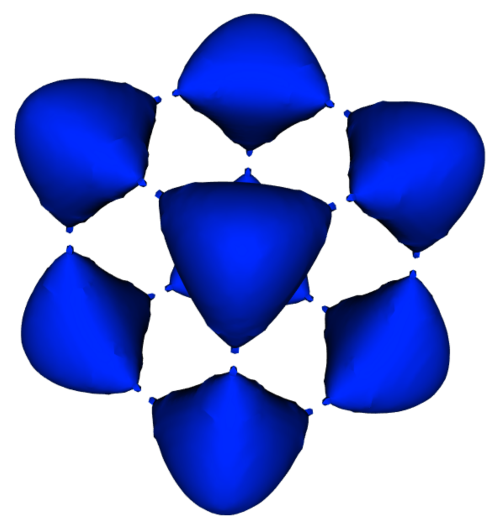
\includegraphics[width=0.85\linewidth]{Images/Tangle/gt.pdf}
\vspace{-2mm}
\caption{Ground truth, $isoval=62$}
\label{fig:tangle_gt}
\end{subfigure}
\begin{subfigure}{0.195\linewidth}
\centering
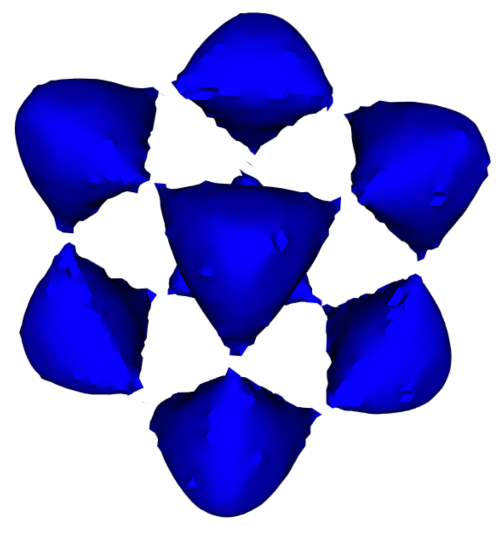
\includegraphics[width=0.85\linewidth]{Images/Tangle/zls.pdf}
\vspace{-2mm}
\caption{$ZLS_{T}$}
\label{fig:tangle_zls}
\end{subfigure}
\begin{subfigure}{0.195\linewidth}
\centering
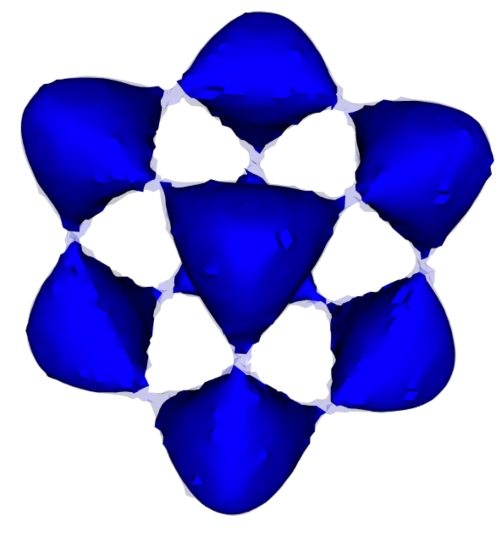
\includegraphics[width=0.85\linewidth]{Images/Tangle/fcls_50.pdf}
\vspace{-2mm}
\caption{$ZLS_{T}$ + $FCLS_{T,50\%}$}
\label{fig:tangle_fcls_50}
\end{subfigure}
\begin{subfigure}{0.195\linewidth}
\centering
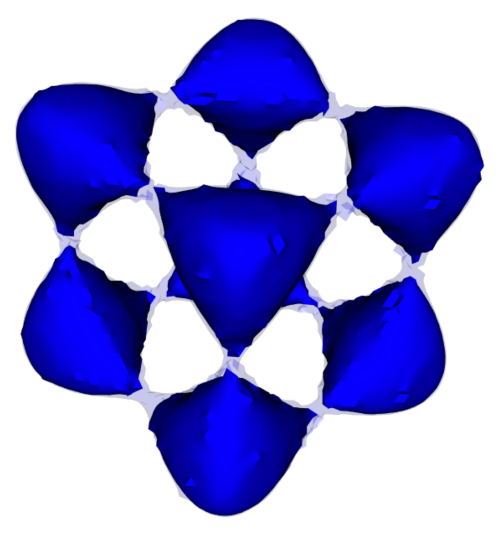
\includegraphics[width=0.85\linewidth]{Images/Tangle/fcls_68.pdf}
\vspace{-2mm}
\caption{$ZLS_{T}$ + $FCLS_{T,68\%}$}
\label{fig:tangle_fcls_68}
\end{subfigure}
\begin{subfigure}{0.195\linewidth}
\centering
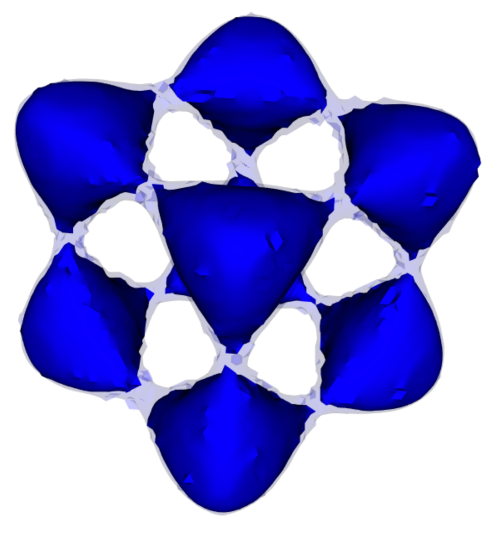
\includegraphics[width=0.85\linewidth]{Images/Tangle/fcls_95.pdf}
\vspace{-2mm}
\caption{$ZLS_{T}$ + $FCLS_{T,95\%}$}
\label{fig:tangle_fcls_95}
\end{subfigure}
%\begin{subfigure}{0.2\linewidth}
%\centering
%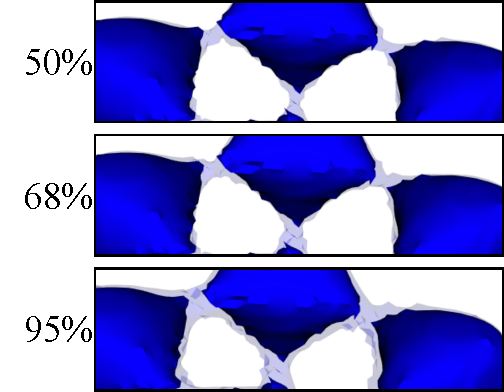
\includegraphics[width=0.8\linewidth, trim={0.5cm 0cm 0.5cm 0cm}, clip]{Images/Tangle/comparison.pdf}
%\vspace{-2mm}
%\caption{Zoomed in comparison.}
%\label{fig:tangle_gt}
%\end{subfigure}
\vspace{-2mm}
\caption{Visualization of sensitivity of the tangle function near values that form links between the multiple blobs. We use $T=[0,62]$.\fix{start a story}}
\vspace{-2mm}
\label{fig:tangle}
\end{figure*}
